\documentclass[12pt,a4paper]{article}

%\usepackage[german]{babel} %Für die indirekte Angabe von Umlauten. Es müssen dann Umlaute wie folgt im Code angegeben werden: "a "o "u "s.

\usepackage[utf8]{inputenc}
%dieses Paket ermöglicht uns, Umlaute im Text als solche eingeben zu können (Windows/Linux)

\usepackage{amsmath, amsthm, amssymb}
\usepackage{enumerate}
\usepackage{graphicx}
\usepackage{lscape}
\usepackage{setspace}
\onehalfspacing
\usepackage{wrapfig}
\usepackage{hyperref}% für die Einbettung von Hyperlinks
\usepackage{multirow}
\usepackage[round]{natbib}
\usepackage{longtable}
\bibliographystyle{apalike}

\newtheorem{definition}{Definition}[section]
\newtheorem{interview}{Interview}[section]
\newtheorem{satz}{Satz}[section]
\newtheorem{beispiel}{Beispiel}[section]
\newtheorem{bemerkung}{Bemerkung}[section]
\newtheorem{literaturverzeichnis}{Literaturverzeichnis}[section]

\usepackage[top=20mm, bottom=20mm, left=20mm, right=20mm, includehead]{geometry} % Document Margins
\setlength{\topmargin}{0cm}
\setlength{\parindent}{0mm}
\setlength{\parskip}{2mm}
\setlength{\evensidemargin}{0mm}
\setlength{\oddsidemargin}{0cm}
%\pagestyle{headings}

\providecommand{\tightlist}{%
  \setlength{\itemsep}{0pt}\setlength{\parskip}{0pt}}

\begin{document}
\thispagestyle{empty}
\vspace*{-3cm}
\begin{center}
\large \textsc{}
\vspace{0.5cm}
%\hrule
\vspace{5.5cm}
{\large}\\
\vspace{1cm}
{\Large \bf
Automatically Estimating Task Durations}\\
\vspace*{1cm}
{\large using arithmetic and artificial intelligence}
\end{center}
\vspace*{14cm}


\hspace*{\fill} from Stefan Hoffmann and others, \today

\newpage
\pagenumbering{Roman}
\tableofcontents

%\newpage
%\addcontentsline{toc}{section}{tables} %wenn es im Inhaltsverzeichnis erscheinen soll - sonst auskommentieren mit "%"
%\listoftables

%\newpage
%\addcontentsline{toc}{section}{Abbildungsverzeichnis} %wenn es im Inhaltsverzeichnis erscheinen soll - sonst auskommentieren mit "%"
%\listoffigures

\newpage
\pagenumbering{arabic}
%Und nun kommen wir zur Arbeit und fangen an die Seiten mit Arabischen Zahlen zu zählen
\hypertarget{foreword}{%
\section{Foreword}\label{foreword}}

I want to make it short. Guessing task durations is a mess. You can put
a lot of effort in making time estimates. Still they will be not good.
And while you strife to make perfect estimates you will find yourself
investing more and more time - possibly a lot more than the task is
worth.

More than that: estimating tasks hurts. Until noone wants to estimate
task durations anymore. It is a pain for developers and business people 
alike.

With automation you can get more benefits and less pain:

\begin{itemize}
\tightlist
\item
  It is clear, that it is just an estimate. Even the most stubborn people have to admit it, because an algorithm just tells you an objective truth and it doesn't really know what it is talking about.
\item
  Algorithms are systematic. Although they do not know what they are actually guessing they are well documented in terms of how they guess. This way they do not trigger the more human problems when guessing time estimates: My boss will half this guess, so I will better double it... Your boss sees your estimate and cuts it down to 15 Minutes because "what could be the problem?": Not a problem anymore.
\item
    And computers can learn from big amounts of data. People can only learn so much, until they are stuck.
\item
  Business people can have their time estimates in real time.
\item
  The developers of those business peoples can do other things in the time they would otherwise need to make "better guesses" (which are also wrong). Most of the time that will mean they code. At since they will probably do that the productivity goes up for the same money.
\item
  The developers are more happy because they do not loose time to guessing and they have no need to fight all the people off that know better.
\end{itemize}

Let us see, if the idea is working or not. Maybe not. But, since the
only thing we have to loose is bad estimates and the only thing we can
gain is bad estimates that do not make effort - what the heck.

\hypertarget{accompagning-material}{%
\section{Accompagning Material}\label{accompagning-material}}

With this booklet I release:

\hypertarget{estimateps}{%
\subsection{EstimatePS}\label{estimateps}}

EstimatePS is a powershell commandlet to estimate tasks from the command
line, implemented but not limited to Powershell Core. The code is part
of this repository. But it is also available through the Powershell
Gallery.

\begin{verbatim}
Install-Module EstimatePS
\end{verbatim}

\newpage{}

\hypertarget{quality-assurance}{%
\section{Quality Assurance}\label{quality-assurance}}

Now if we create algorithms we need to say how good they are. For that
we are using the following methods.

\hypertarget{the-graphical-approach}{%
\subsection{The graphical approach}\label{the-graphical-approach}}

One easy way would be to draw a graph which shows the predictions and
the real values for time spent, while each task is understood as a
category of its own.

We sort that graph by actual duration so we should see the distribution
of durations and around that a hopping range of dots that describes what
the algorithm tells us.

A better algorithm should be closer to the real data. Any algorithm
should never match perfectly, as then we would have a 1:1 mapping. And
that is an over-fit for sure.

\hypertarget{mean-squared-error}{%
\subsection{Mean squared error}\label{mean-squared-error}}

The mean squared error is a common approach to calculate a value for the
quality of an algorithmi. It gets bigger with every estimate we did
wrong.

The formula can be described as:

For every value you predict:

\begin{itemize}
\tightlist
\item
  Calculate the difference between the predicted value and the real
  value
\item
  Sum the squares of each difference
\item
  Divide all the sum by the count of the data entries you check
\end{itemize}

Now, since we want to prevent overfitting we need to prevent
underfitting as well. Since we are talking about seconds and most of the
recorded tasks have a duration in the range of up to 50000 seconds that
means that most tasks are completed in about 13,89 hours. So what about
an error margin of about 5 hours. Which means just as something to think
of, we want the squared error to not exceed squared(5x60x60) =
324.000.000 .

\hypertarget{above-and-below}{%
\subsection{Above and below}\label{above-and-below}}

As a third criteria we have the idea that estimations might even each
other out. In a prefect scenario this would mean that 50\% of the
estimations are too high while the other 50\% are too low. To find out
how good we match we add 1 to a variable for every estimation we find
above the real value and then divide it by the number of tasks. The
result should be .5 when hitting the target.

\hypertarget{the-data}{%
\subsection{The Data}\label{the-data}}

For training and estimating the quality of algorithms I use herein a
dataset that consists of all the tasks that we at the software
development shop at my employer recorded during the time between july
and december 2020 and january 2021 to august 2021. That means there are
two datasets available.

Unfortunately - since this is confidential information - I cannot
publish it alongside this material. But the errors and images can be
shared at it can advance the algorithms - and it is everything that I
have right now. So that will do.

I'll call them: swe2020 and swe2021.

Now let us get a glance at the data as well the first algorithm.


\newpage{}

\hypertarget{a001---duration-per-word}{%
\section{A001 - Duration per Word}\label{a001---duration-per-word}}

\hypertarget{description}{%
\subsection{Description}}

Let us dive in with a very very simple algorithm. In fact it is the
first algorithm I tought of.

Let's say we have a task. May it read ``Buy a big book and put it in the
shelf''. And this takes a certain amount of time.

\begin{verbatim}
AmountOfTime = "Buy a big book and put it in the shelf"
\end{verbatim}

Ok, I know, language doesn't really work like that. But lets us play
stupid right now. We just split the thing into words and distribute the
duration equally to each word. The sentence above is 10 words long, so
each word gets a tenth of AmountOfTime associated with it.

Now we have a minimal time table.

We can now take another input, like ``Buy a small book''.

We know the durations associated with ``Buy'', ``a'' and ``book''. We
will have to do something about the unknown word. Ignore it, or add 10\%
to the sum of the known durations. Something like that. And voilà, we
have a time estimate.

Funny thing:

It is actually quite reasonable for the time being, that, in the absence
of further information, assigning half the duration to each subtask is
not the most stupid thing one could do.

And it is actually quite reasonable to think that buying a small book is
about the effort of buying a big one. But that is just the example.

Anyways, we now have a time estimate and noone got hurt.

\hypertarget{using-the-algorithm-from-powershell}{%
\subsection{Using the algorithm from powershell}}

The algorithm is added to EstimatePS, see
Source/experiments/duration-per-word/experiment1.ps1 for a complete
example with learning, caching and usage.

Finally it is as easy as:

\begin{verbatim}
$inSeconds = Get-DPWEstimate -Model $model -DurationInSecondsFor "add a new bookkeeping api" -ProbabilityInPercent 95
\end{verbatim}

\hypertarget{how-good-is-it}{%
\subsection{How good is it?}}

As you can see there is a parameter in the algorithm, the ``probability
in percent'' which decides if it should tend to higher values or not.
Since it has influence and we want to know what that influence looks
like I will use three different values for this validation: 25\%, 50\%
and 75\%.

\begin{figure}
\centering
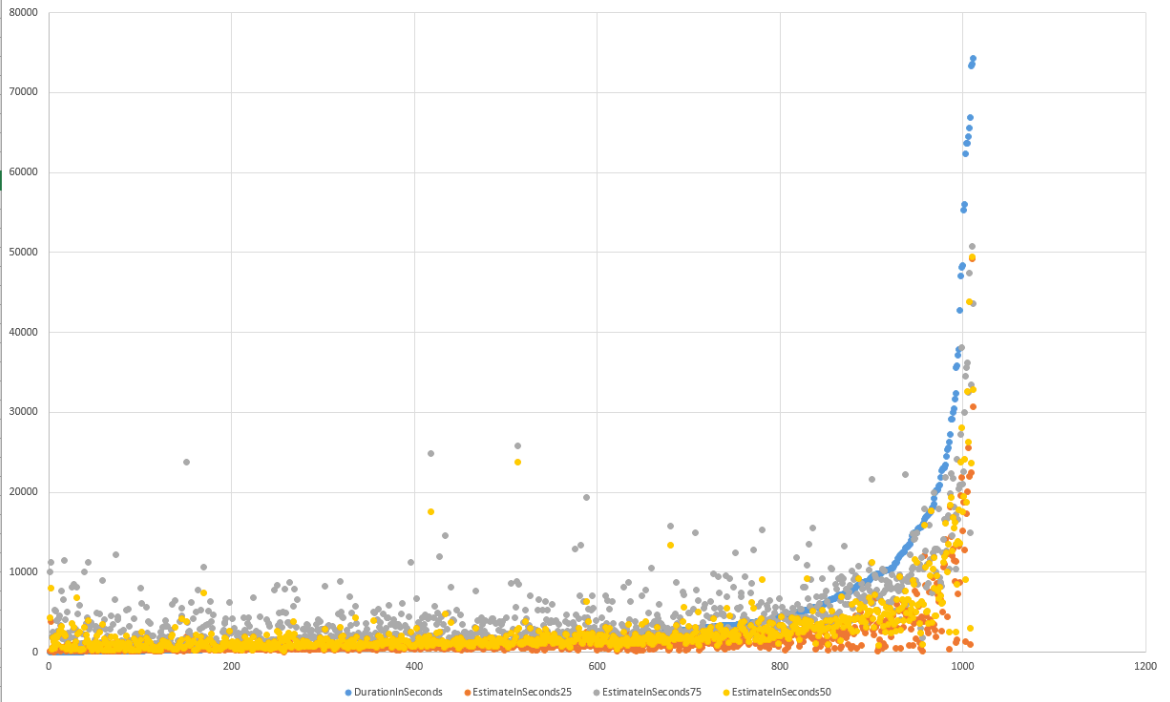
\includegraphics[width=\textwidth]{Documentation/10000-A001/a001-swe2020.png}
\caption{QA a001 - swe 2020}
\end{figure}

\begin{longtable}[]{@{}lll@{}}
Probability & Mean squared error & Percent guesses above real
duration\tabularnewline
\endhead
25\% & 46.205.433 & 20,96\%\tabularnewline
50\% & 35.826.104 & 51,33\%\tabularnewline
75\% & 28.595.545 & 76,75\%\tabularnewline
\end{longtable}

Our target mean squared error is 324.000.000 One hour is about 12.9 mio
square seconds. Two hours is about 51.8 mio square seconds. That means
that our error marin is about two hours here.

But this is the data we trained the model on, the 2020 tasks below
100000 seconds (which trims off only 12 tasks from more than 1000).

Now let us see how it performs on the 2021 tasks below 100000 seconds:

\begin{figure}
\centering
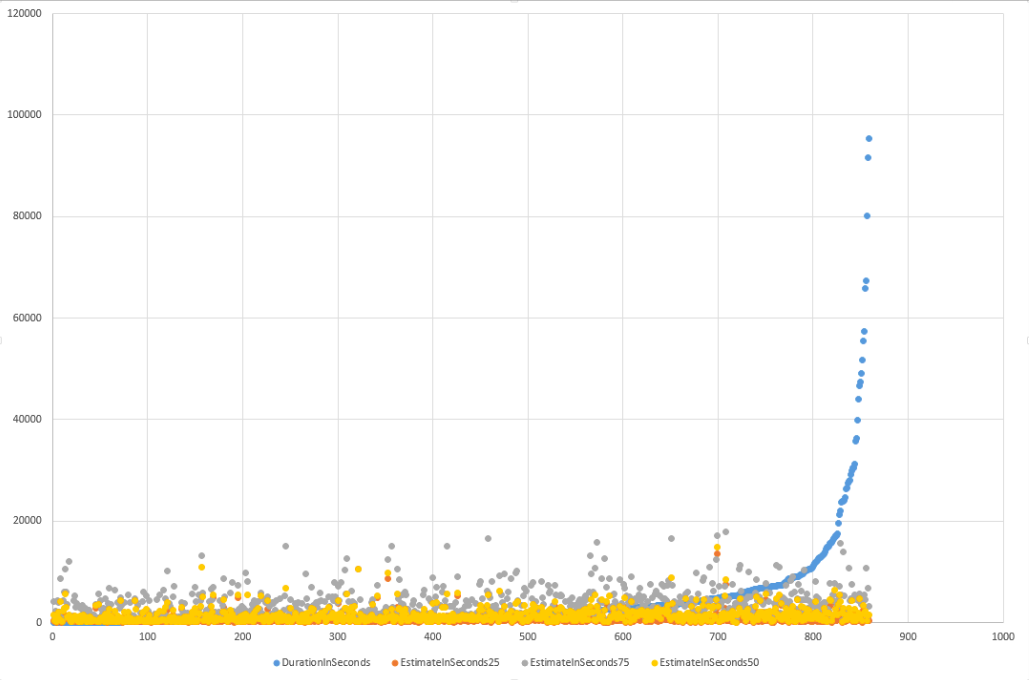
\includegraphics[width=\textwidth]{Documentation/10000-A001/a001-swe2021.png}
\caption{QA a001 - swe 2021}
\end{figure}

\begin{longtable}[]{@{}lll@{}}
Probability & Mean squared error & Percent guesses above real
duration\tabularnewline
\endhead
25\% & 88.106.182 & 25,96\%\tabularnewline
50\% & 84.227.983 & 45,52\%\tabularnewline
75\% & 80.881.803 & 70,20\%\tabularnewline
\end{longtable}

We are still below our 5h target which makes the algorithm still
acceptable, although the error margin is higher now.

\newpage{}
\newpage{}

\hypertarget{a002---simply-an-average}{%
\section{A002 - Simply an average}\label{a002---simply-an-average}}

\hypertarget{description}{%
\subsection{Description}\label{description}}

Another algorithm could just calculate an average. Take all tasks and
their durations, divide them by their count. Is this better?

From visually reviewing the data we know that most tasks have a duration
of a few hours max. Some take very long.

An average is not just an average as we know. There are several ways to
calculate one:

\begin{itemize}
\tightlist
\item
  there is the ``simple average'' that includes all data (A002.1)
\item
  there is the possibility of a boxplot like calculation, include only
  the middle n\% of the values (A002.2)
\end{itemize}

\hypertarget{using-the-algorithm-from-powershell}{%
\subsection{Using the algorithm from
powershell}\label{using-the-algorithm-from-powershell}}

\hypertarget{a002.1}{%
\subsubsection{A002.1}\label{a002.1}}

Have a look at Quality-Assurance\_A002\_1\_swe2020.ps1 if you need more.
But actually it is just calculating the average. It is not even
necessary to do this in a programming language alltogether.

\begin{verbatim}
$averageTaskDuration = ($historicData.DurationInSeconds | Measure-Object -Average).Average

$anyEstimation = $averageTaskDuration
\end{verbatim}

\hypertarget{a002.2}{%
\subsubsection{A002.2}\label{a002.2}}

For that average let us only use the middle 90\% of duration values.
That will cut extreme points and should reduce the error.

Quality-Assurance\_A002\_2\_swe2020.ps1:

\begin{verbatim}
$historicData = $historicData | Sort-Object DurationInSeconds
$count = ($historicData | Measure-Object).Count
$fivePercent = [int]($count * 0.05)
$historicData = $historicData[$fivePercent..($count-$fivePercent)]
\end{verbatim}

\hypertarget{how-good-is-it}{%
\subsection{How good is it?}\label{how-good-is-it}}

\hypertarget{a002.1-1}{%
\subsubsection{A002.1}\label{a002.1-1}}

\textbf{on swe2020 data}

Mean squared error: 765.929.757 Percent of estimates that are too high:
83,68 \%

\begin{figure}
\centering
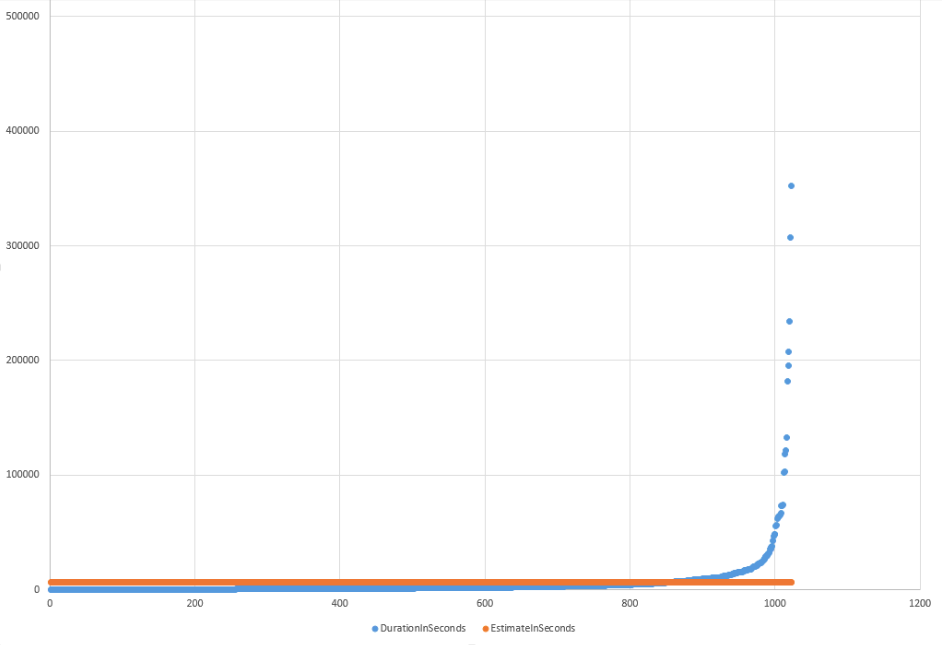
\includegraphics{Documentation/10000-A002/a002_1-swe2020.png}
\caption{QA a002.1 - swe 2020}
\end{figure}

\textbf{on swe2021 data}

Mean squared error: 321.140.140 Percent of estimates that are too high:
85,55 \%

\begin{figure}
\centering
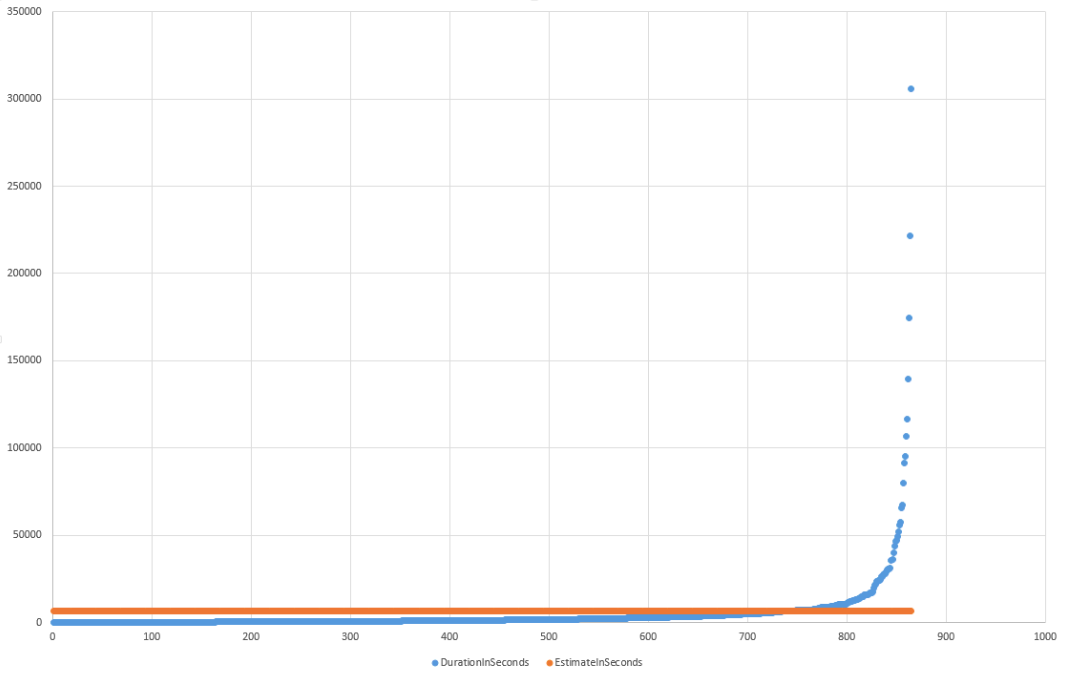
\includegraphics{Documentation/10000-A002/a002_1-swe2021.png}
\caption{QA a002.1 - swe 2021}
\end{figure}

\hypertarget{a002.2-1}{%
\subsubsection{A002.2}\label{a002.2-1}}

\textbf{on swe2020 data}

Mean squared error: 780.036.288 Percent of estimates that are too high:
69,01 \%

\begin{figure}
\centering
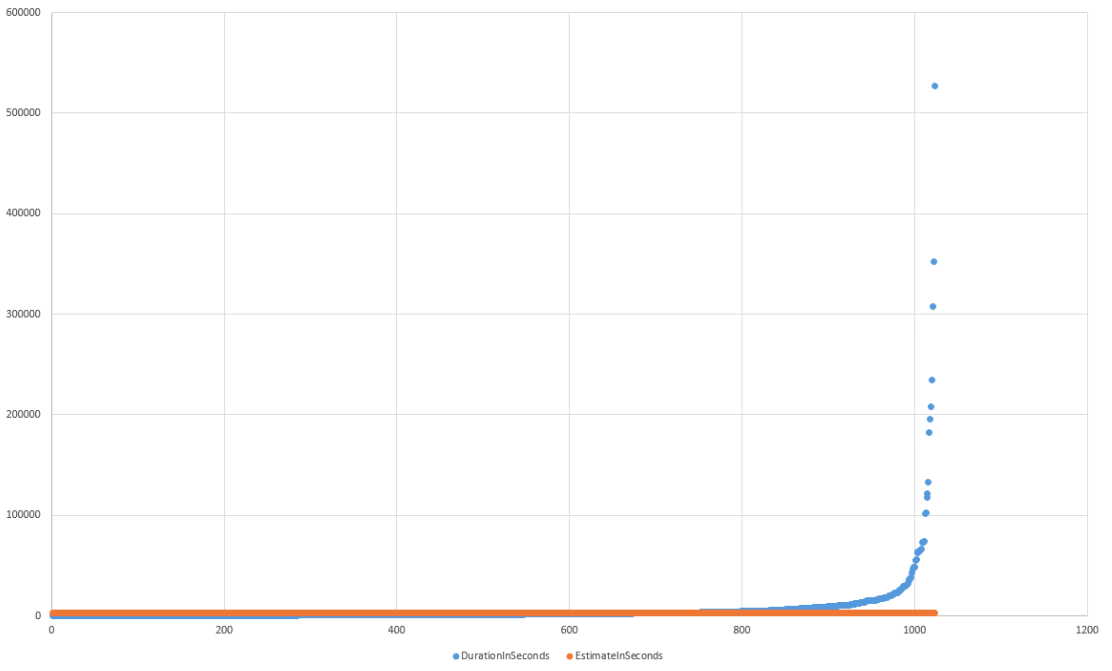
\includegraphics{Documentation/10000-A002/a002_2-swe2020.png}
\caption{QA a002.2 - swe 2020}
\end{figure}

\textbf{on swe2021 data}

Mean squared error: 323.888.830\\
Percent of estimates that are too high: 69,94 \%

\begin{figure}
\centering
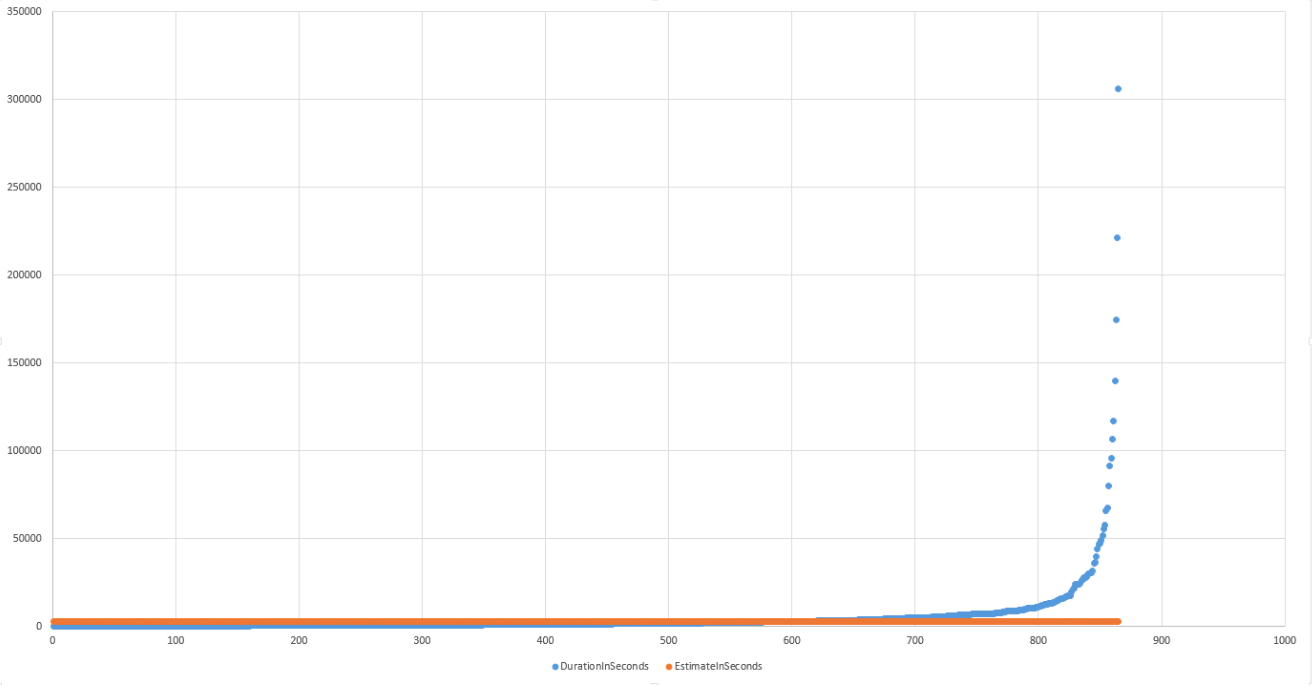
\includegraphics{Documentation/10000-A002/a002_2-swe2021.png}
\caption{QA a002.2 - swe 2021}
\end{figure}

\newpage{}

\hypertarget{a003---10-categories}{%
\section{A003 - 10 categories}\label{a003---10-categories}}

\hypertarget{description}{%
\subsection{Description}}

To be better than A001 we could use a categorization.
For that we divide all tasks into 10 groups with similarities. 
Our target here is to reduce the dispersion within those groups. E.g. we know that there are a lot of tasks below half an hour duration. A001 often claims they are more costly. If we could clearly say that a task would belong to that category we could reduce our error margin here.
But how can we accomplish that?

\subsubsection{A003.1}

We divide our tasks using a linear scale
\begin{enumerate}
\tightlist
\item smaller than 30 minutes,
\item bigger than 30 minutes and less than one hour,
\item bigger than 1 hour and less than 2 hours
\item bigger than 2 hour and less than 3 hours
\item bigger than 3 hour and less than 4 hours
\item bigger than 4 hour and less than 5 hours
\item bigger than 5 hour and less than 6 hours
\item bigger than 6 hour and less than 7 hours
\item bigger than 7 hour and less than 8 hours
\item bigger than 8 heures
\end{enumerate}

Our algorithm tries to identify significant words that are unique par category:
\begin{enumerate}
\tightlist
\item collect all words in a category
\item for all categories:
    \begin{enumerate}
        \tightlist
        \item remove all words that are somehow mentioned in another category
    \end{enumerate}
\end{enumerate}
\newpage{}

\section{A004 - reducing dispersion by assigning a concrete value per
word and learning from
it}

A001 collects as many different values for each word as it can get. 
When estimating, it uses any of those values more or less randomly (of cause
smoothend by the fact that we take 100 random values and then only use a
value from a certain position representing the percentage of certainty
we want to have). 
That hinders our ability to ``learn''.

The idea behind A004 is to assign just one value to each word.
This way, when we see our error margin we might design a little learning by adding or reducing the values a bit and see what happens.

\subsection{Learning - the Initialisation}

At the beginning we learn just the same way like A001 did.
The only difference is, that instead of saving n values per word we just save one, the average of all beformentioned values. 

\subsection{Learning - Adapting}

\begin{enumerate}
        \tightlist
        \item starting from the base model we create 10 mutations by randomly adding and substracting 1/10th of the value for each word.
        \item we calculate the mean squared error of all mutations
        \item the mutation with the smallest mean squared error becomes the new base model
        \item repeat n times from the beginning
\end{enumerate}

\subsection{Estimating}

\begin{enumerate}
        \tightlist
        \item split the text we want to estimate into words
        \item for every word use the saved value as duration
        \item add all values gained this way, the sum is our estimate
\end{enumerate}




\end{document}

